\newcommand{\id}{\schemefont{id}}
\begin{figure}
  \twoColsNoDivide{0.22}
  {
    \underline{$\Rep^R_K(\col)$}\\[2pt]
      if $|\col| > n$ return $\bot$\\
      $\salt \getsr \bits^\lambda$\\
      $M \gets \bigvee_{x \in \col} \bmap_m(R_K(\salt \cat x))$\\
      return $\langle M, \salt \rangle$
  }
  {
    \underline{$\Qry^R_K(\langle M, \salt \rangle,x)$}\\[2pt]
      $X \gets \bmap_m(R_K(\salt \cat x))$\\
      return $M \AND X = X$
    \\[6pt]
    \underline{$\Up^R_K(\langle M, \salt \rangle,x)$}\\[2pt]
      if $\hw(M) > \ell$ then return $\bot$\\
      return $\langle M \vee \bmap_m(R_K(Z \cat x)), \salt \rangle$
  }
  \caption{The keyless structure $\bloom[R,\ell,n,\lambda]$ given by
  $(\Rep^R,\Qry^R,\Up^R)$ is used to define Bloom filter variants. The
  parameters are a function $R: \keys\by\bits^* \to [m]^k$ and integers $\ell, n,
  \lambda \geq0$. A concrete scheme is given by a particular choice of
  parameters.  Functions~$\hw$ and~$\bmap_m$ are defined in
  Section~\ref{sec:prelims}.
  }
  \label{fig:bf-def}
\end{figure}

\todo{Any}{This should be moved to Section~\ref{sec:prelims}.}

\heading{Bitstring operations}
%
For all $m\geq0$ define~$\bmap_m$ as the following function.
For all $\v.x\in[m]^*$ let $\bmap_m(\v.x) = X$, where
$|X|=m$ and $X_v=1$ if and only if $\v.x_i = v$ for some $i\in[|\v.x|]$
%
We call $\bmap_m(\v.x)$ the \emph{bitmap} of~$\v.x$.
%
Let~$X$ and~$Y$ be equal-length bitstrings. We write $X \OR Y$ for their
bitwise-OR, $X \AND Y$ for their bitwise-AND, and $X \XOR Y$ for their
bitwise-XOR. Let $\NOT X = 1^{|X|} \xor X$.
%
Finally, let $\hw(X)$ denote the Hamming wieght of (i.e., the number of 1s in)~$X$.

\heading{More prliminaries}
%
For every function~$f$, define function $\id^f$ so that
$\id^f(\emptystr, x) = f(x)$ for all $x$ in the domain of~$f$.

\medskip
We specify three Bloom filter variants using the keyed structure
$\bloom[R,\ell,n,\lambda] = (\Rep^R,\Qry^R,\Up^R)$ specified in
Figure~\ref{fig:bf-def}.
%
The construction has four paraemters: a function~$R:\keys\by\bits^*\to[m]^k$, the
\emph{update threshold} $\ell\geq0$, the \emph{initial threshold} $n\geq0$, and
the \emph{salt length}~$\lambda\geq0$.
%
Let $H:\bits^*\to[m]^k$ be a hash function and let $\ell, n, \lambda\geq0$ be
integers.
%
The standard Bloom filter is the structure $\BF[H,\ell,n] =
\bloom[\id^H,\ell,n,0]$, which we will term the \emph{basic} Bloom filter. It
has no key (the key sapce of $\id^H$ is $\{\emptystr\}$, see
Section~\ref{sec:prelims}) and does not use a salt.
%
The \emph{salted} Bloom filter $\SBF[H,\ell,n,\lambda] =
\bloom[\id^H,\ell,n,\lambda]$ is the same except that it allows a nonempty salt.
%
Finally, we also consider a salted variant that uses a PRF instead of a hash
function. The \emph{keyed} Bloom filter $\KBF[F,\ell,n,\lambda]$ is the
structure $\bloom[F,\ell,n,\lambda]$, where $F:\keys\by\bits^*\to[m]^k$ is a
PRF.
%
Note that the basic and salted BFs have key spaces $\{\emptystr\}$ and the keyed
BF has key space~$\keys$.

\todo{DC (lead)}{Summarize the results of this section: unsalted is bad; salted
is OK for immutable filters; salted, secret rep is OK for mutable filters; and
...}
\ignore{%
The standard Bloom filter shows a variety of different behaviors depending on
its exact implementation. If the hash functions used are chosen beforehand and
potentially known to the adversary, this public information allows offline
attacks to be mounted against the data structure which can produce potentially
damaging false positives. In the case of immutable Bloom filters, making use of
a per-representation salt is sufficient to prevent these attacks, though
depending on the use case the use of non-fixed per-representation randomness may
or may not be feasible. Furthermore, in the case of mutable Bloom filters there
are additional difficulties with offline attacks due to adversarially-chosen
updates. To guarantee correctness in this case we must additionally guarantee
that representations can be kept private from the adversary.
}

\heading{Error function for set-mempership queries}
%
\todo{DC (lead)}{Decide if this is a sutiable function.}
%
Throughout this section we will use the error function $\delta:\bits^2\to\N$
defined as
\begin{equation*}
  \delta(a, b) =
  \begin{cases}
    1 & \text{if}\ a=b \\
    0 & \text{otherwise.}
  \end{cases}
\end{equation*}

\subsection{Insecurity of unsalted BFs}
Fix a hash function $H:\bits^*\to[m]^k$ and integers $\ell,n\geq0$ and let $\Pi
= \BF[H,\ell,n] = (\Rep^H, \Qry^H, \Up^H)$.
%
Suppose the adversary is interacting with a system representing a dataset
with~$\Pi$ and that it is able to choose some fraction of the input data.
%
\todo{DC (lead)}{Pick a concrete attack setting, like a CDN. ``For example
...''.}

\heading{Pollution attacks}
%
The goal of the attacks pointed out by Gerbet \etal~~\cite{gerbet2015power} is
to pollute the filter such that the ``average'' set-membership query yields a
false positive with high probability; to do so, the attacker chooses a set of
inputs that maximize the number of 1s in the filter. This strategy is especially
effective when the structure of the hash function can be exploited.
%
\todo{DC (lead)}{Add a brief summary of attacks of Gerbet \etal that exploit bad
choices of hash functions. What fraction of the inputs does the adversary need
to control for the attack to be effective?}
%
Pollution attacks can even even be damaging for ``good'' choices of hash
functions, but their effectiveness depends crucially on the fraction of inputs
controlled by the adversary.
%
\todo{DC (lead}{Verify this claim. and discuss Gerbet \etal's mitigations of
pollution attacks.}

\heading{Target-set coverage attacks}
%
Of course, exhibiting a high false positive rate is not the only way a Bloom
filter might fail to be correct. In particular, it would be undesirable if the
filter were consistently incorrect on a \emph{particular set of inputs}. Rather
than pollute the filter, the adversary's goal might be to craft a set of
legitimate looking inputs that cover some disjoint target set of inputs.
%
This type of attack is nicely captured by our adversarial model.
%
In a \emph{target-set coverage attack}, the adversary is given a small target set
$\setT\subseteq\bits^*$ and searches for a cover set $\setR\subseteq\bits^*$
such that $\Qry^H(\Rep^H(\setR),x)=1$ for each $x\in\setT$.
%
Once a suitable cover set is found, the adversary queries $\Rep(\setR)$. Then
for each $x\in\setT$, it asks $\Qry(x)$, achieving a score of $r = |\setT|$.

This \erreps1 attack succeeds with probability~$1$ assuming a covering set can
be found.  If $|\setT| \leq |\setR|$, then such a set exists; but finding it may be
computationally infeasible, depending on the size of the cover set, the size of
the target set, and the parameters of the Bloom filter.
%
In Appendix~\ref{app:unsalted-attack} we demonstrate that target-set coverage
attacks are feasible for practical BF parameters. We do so by simulating the
attack when~$H$ is a random function (i.e., for each distinct input we choose
$k$ integers from $[m]$ at random) for typical choices of $k$, $m$, and~$n$.
%
\todo{CP}{Add simulation to appendix.}

\todo{DS (lead)}{Double check that Gerbet \etal don't suggest anything like this
attack. If they do it's not a big deal; we just need to ensure, to the best of
our ability, that we give credit where credit is due.}

The key to pollution attacks and target-set coverage attacks is that the
adversary can compute the representation of the set on its own. In the remainder
of this section, we examine ways of enhancing the basic BF structure so that it
avoids this pitfall.

\subsection{Salted BFs in the (im)mutable setting}
%
Here we consider the correctness of Bloom filters when the hashed input is
prepended with a salt.
%
Fix $H:\bits^*\to[m]^k$, $\ell,n,\lambda\geq0$, and let
$\Pi = \SBF[H,\ell,n,\lambda] = (\Rep^H, \Qry^H, \Up^H)$ as defined above.

The security of this structure depends upon how it is used.
%
\todo{DC (lead)}{As concisely as you can, articulate the \errep\ attack against~$\Pi$.
Remember that the adversarial model (i.e., the security experiment) is supposed
to reflect how the primitive is supposed to be used. So when giving attacks, try
to make it clear what the attack is. You should answer the following questions:
What is the sequence of queries made by the adversary?
How efficient is the attack?
Is the attack devastating? Is it a real attack, or is it more theoretical?
What about the scheme and setting make it possible?
%
Note that I've left your text in a ignore\{\} so that you can lift from it as
needed.
}\ignore{
The use of a salt without a private key in the \errep\ setting is
insufficient to defeat [the attacka above]. In this setting, the adversary need only
make its $\REPO$ query for $\setT$ in advance, at which point it will receive
both the representation $\pub$ and the salt $\salt$ used to construct it. Using
this known salt, the adversary is still able to simulate $\REPO$ for arbitrary
singleton representations. The previous attack therefore still works with the
same (minimal) number of $\QRYO$ calls at the very end of the experiment, after
it has determined $\setR$ using offline computations.
\cpnote{I don't think this is true, since each $\ROPO$ query returns a filter
with a different, independently generated salt.}

The opposite of this, using a private key without a salt, does weaken the attack
somewhat. Even with public representations, the adversary cannot locally
simulate $\REPO$ without guessing the private key. However, they can still
outperform random $\QRYO$ calls by making $\REPO$ queries for singleton elements
without fixing any $\setT$ in advance. After selecting a random set $\col$ of
size $q_R-1$, the adversary performs offline computations to find $\setT$,
$\setR \subseteq \col$ such that the elements of $\setR$ are false positives for
the representation of $\setT$ (which can be computed from the representations of
the singleton subsets of $\setT$). The adversary wins if there is a partition
where $\setR$ produces at least $r$ errors on $\REPO(\setT)$.
\cpnote{This might be the case, but I don't think it's worth spending too much
time on. We're going to have other reasons for needing to add salt even when
there's a key.}

Using a salted Bloom filter in the private representation setting, however, does
provide some security. At the time a representation is created, the structure
chooses a salt $\salt$ which it will use for all further queries and updates. In
order for maximum security to be guaranteed, we must ensure that the
representation, and in particular the salt, is kept secret from the adversary.
We define this structure $\SBF[H,k,m,n,\lambda]$ as the Bloom filter structure
that uses $H(s) = (h_1(s),\ldots,h_k(s))$ for hashing inputs to $k$ values in
$[m]$. Furthermore, each call of $\Rep$ first involves picking a salt $\salt$
from the salt space $\bits^\lambda$, and all hashes made to insert or query for
an element $x$ are determined using $H(x \Vert \salt)$. Finally, the parameter
$n$ means that any attempts to represent sets with more than $n$ elements fail.
\todo{DC lead}{Specify what exactly is being analyzed.  What are the updates?}
}

The above attack exploits the mutability of~$\Pi$ in a crucial way.
%
\todo{DC (lead)}{Verify this, and remind the reader of what that ``crucial''
thing is.}
%
Indeed, when restrict ourselves to the immutable setting, we can prove the
following.
%
\begin{theorem}[\errep1 security of salted BFs]\label{thm:sbf-errep1}
  For integers $q_R, q_T, q_H, r, t \geq 0$ it holds that.
  \begin{equation*}
    \begin{aligned}
      \Adv{\errep1}_{\Pi,\delta,r}(t, q_R,q_T,q_H) &\leq \\
      \hspace{20pt}
        \text{some cool bound} \,,
    \end{aligned}
  \end{equation*}
  where $H$ is modeled as a random oracle.
  %
  \cpnote{I'm not sure if this advantage function is defined.}
\end{theorem}
\begin{proof}
  We will use the following lemma for keyless structures.
%
\todo{DC (lead)}{Prove this,}

\begin{lemma}\label{thm:lemma1}
  For every $q_R, q_T, q_U, q_H, r, t \geq 0$ and keyless structure~$\Gamma$ it
  holds that
  \begin{equation*}
    \Adv{\errep}_{\Gamma,\delta,r}(t, q_R, q_T, q_U, q_H) \leq
    q_R\Adv{\errep1}_{\Gamma,\delta,r}(O(f(t)), q_T, q_U, q_H) \,,
  \end{equation*}
  where $f(t) = t + (q_R-1)\ticks(\Rep,t) + q_T\ticks(\Qry,t) + q_U\ticks(\Up,t)$.
  \todo{Any}{Define $\Adv{\errep1}_{\cdot,\cdot,\cdot}(\cdots)$.}
\end{lemma}
%
%
\noindent
The proof is by a fairly straight-forward hybrid argument. Because~$\Gamma$ is
keyless, in the reduction we simulate $q_R-1$ $\REPO$-queries experiment and use
our own oracles for the remaining query. The best we can do with this strategy
is to ``guess'' which representation the \errep\ adversary willl use in its
attack, which results in the~$q_R$ factor in the bound.
%
We defer the full details to Appendix~\ref{app:iproof/lemma1}.

Let $\advA$ be an \errep\ adversary making~$1$ query to~$\REPO$, $q_T$ queries
to $\QRYO$, $0$ queries to $\UPO$, and $q_H$ queries to the random
oracle~$\HASHO$.
%
We assume, without loss of generality, that all of~$\advA$'s $\QRYO$ queries
proceed its $\REPO$ query, for each query $\qry_x$ to  

\ignore{

The proof is by a game-playing argument~\cite{bellare2006triple}.

Let $\struct_\saltybloom = (\Rep, \Qry)$.
%
We define a deterministic algorithm, $\Repx$, that on input of a
collection~$\col$ and salt~$\salt$ computes the Bloom filter
representation of~$\col$ and outputs~$\str(M, \salt)$.
%
(Then running $\salt \getsr \bits^\lambda$ followed by $\pub \gets
\Repx^H(\col, \salt)$ is equivalent to running $\pub \getsr \Rep^H(\col)$.)
%
Define the function~$\fff$ from $[m]^2$ to $[m]^k$ as $\fff(\hh)=\vv$, where
$\vv_j = 1 + (\hh_1 + j\cdot\hh_2 \mod m)$ for each $j\in[k]$.
%
Let~$\advA$ be an \errepone adversary. Let~$q_1$ denote the number of
queries~$\advA$ makes to~$H$ during its first stage, let $q_2$ denote the number
of queries during its second stage, and let~$q_T$ denote the number of queries
to~$\QRYO$.
%
We assume that none of the adversary's queries coincide with the collection,
meaning for every query~$\qry_x$ that~$\advA$ asks of its~$\QRYO$ oracle,
it holds that~$x \not\in \col$. This is without loss of generality; since
Bloom filters never have false negatives, the adversary can compute the result
of these queries without interacting with its oracle.

\begin{figure*}
  \boxThmBFSaltCorrect{0.48}
  {
    \underline{$\game_0(\advA)$}\\[2pt]
      $\col \getsr \advA^H$; $\setC \gets \emptyset$; $\err \gets 0$\\
      $\pub \getsr \Rep[\hashbf[H]](\col)$\\
      $\bot \getsr \advA^{H,\QRYO}(\pub)$;
      return $(\err \geq r)$
    \\[6pt]
    \oraclev{$\QRYO(\qry_x)$}\\[2pt]
      if $\qry_x \in \mathcal{C}$ then return $\bot$\\
      $\setC \gets \setC \union \{\qry_x\}$\\
      $a \gets \Qry[\hashbf[H]](\pub, \qry_x)$\\
      if $a \neq \qry_x(\col)$ then $\err \gets \err + 1$\\
      return~$a$
    \\[4pt]
    \hspace*{-4pt}\rule{1.043\textwidth}{.4pt}
    \\[5pt]
    \oraclev{$\HASHO_1(\salt,x)$} \hfill\diffplus{$\game_2$}\;{$\game_1$}\hspace*{3pt}\\
      $\hh \getsr [m]^2$; $\vv \gets \fff(\hh$)\\
      if $\salt = \salt^*$ then\\
      \tab $\bad_1 \gets 1$; \diffplus{return $\vv$}\\
      if $T[\salt,x]$ is defined then $\vv \gets T[\salt,x]$\\
      $T[\salt,x] \gets \vv$;
      return $\vv$
  }
  { % New RO semantics
    % Change of hashing scheme (iid since inputs are distinct)
    \underline{$\game_1(\advB)$}\\[2pt]
      $\salt^* \getsr \bits^\lambda$;
      $\col \getsr \advB^{\HASHO_1}$\\
      $\pub \gets \Repx[\HASHO_2](\col, \salt^*)$\\
      $\setC \gets \emptyset$;
      $\err \gets 0$\\
      $\bot \getsr \advB^{\HASHO_3,\QRYO}(\pub)$;
      return $(\err \geq r)$
    \\[6pt]
    \oraclev{$\QRYO(\qry_x)$}\\[2pt]
      if $\qry_x \in \mathcal{C}$ then return $\bot$\\
      $\setC \gets \setC \cup \{\qry_x\}$\\
      $a \gets \Qry[\HASHO_3](\pub, \qry_x)$\\
      if $a \neq \qry_x(\col)$ then $\err \gets \err + 1$\\
      return~$a$
    \\[6pt]
    \oraclev{$\HASHO_i(\salt,x)$}\\[2pt]
      $\hh \getsr [m]^2$; $\vv \gets \fff(\hh$)\\
      if $\salt = \salt^*$ then $\bad_i \gets 1$\\
      if $T[\salt,x]$ is defined then\\
      \tab $\vv \gets T[\salt,x]$\\
      $T[\salt,x] \gets \vv$;
      return $\vv$
  }
  {
    \underline{$\game_3(\advB)$}\\[2pt]
      $\salt^* \getsr \bits^\lambda$;
      $\col \getsr \advB^{\HASHO_1}$\\
      $\pub \gets \Repx[\HASHO_2](\col, \salt^*)$\\
      $\setC \gets \emptyset$;
      $\err \gets 0$\\
      $\bot \getsr \advB^{\HASHO_3,\QRYO}(\pub)$;
      return $(\err \geq r)$
    \\[9pt]
    \oraclev{$\QRYO(\qry_x)$}\\[2pt]
      if $\qry_x \in \setC$ then return $\bot$\\
      $\setC \gets \setC \union \{\qry_x\}$\\
      if $\Ans[x]$ is undefined then\\
      \tab $\vv \gets \HASHO_3(\salt^*,x)$\\
      return $\Ans[x]$
  }
  {
    \oraclev{$\HASHO_3(\salt,x)$}\\[2pt]
      $\hh \getsr [m]^2$; $\vv \gets \fff(\hh$)\\
      if $T[\salt,x]$ is defined then\\
      \tab $\vv \gets T[\salt,x]$\\
      $T[\salt,x] \gets \vv$\\
      if $\salt \ne \salt^*$ or $\qry_x \in \setC$ then return~$\vv$\\
      $\setC \gets \setC \union \{\qry_x\}$\\
      $\Ans[x] \gets 1$;
      for $j \gets 1$ to $k$ do\\
      \tab\tab if $M[\vv_j] \neq 1$ then $\Ans[x] \gets 0$\\
      if $\Ans[x] \ne \qry_x(\col)$ then\\
      \tab $\err \gets \err + 1$\\
      return $\vv$
  }
  \caption{Games 0--3 for proof of Theorem~\ref{thm:bf-salt-correct}.}
  \label{fig:bf-salt-correct}
  %\vspace{6pt}
  %\hrule
\end{figure*}

The proof is by a game-playing argument; see Figure~\ref{fig:bf-salt-correct}.
%
Game~$\game_0$ is precisely the \errepone game with~$\struct_\saltybloom$,
adversary~$\advA$, and error parameter~$r$, and so
$\Adv{\errepone}_{\struct_\saltybloom,r}(\advA) = \Prob{\game_0(\advA)=1}$.
%
Next, $\game_1$ differs from~$\game_0$ in three important ways.
%
First, the random oracle~$H$ is replaced with three oracles: $\HASHO_1$ is
given to the adversary's first stage, $\HASHO_2$ is used to compute the
representation, and $\HASHO_3$ is given to the adversary's second stage and
is also used by~$\Qry$ to answer the $\QRYO$ queries.  All of them
populate the same table~$T$ mapping inputs to random values, thereby simulating
a single random oracle via lazy evaluation.
%
Second, whereas~$H$ maps strings to $[m]$, oracles $\HASHO_1$,
$\HASHO_2$, and $\HASHO_3$ map elements of $\bits^\lambda \cross
\bits^*$ to $[m]^k$.
%
Third, the salt~$\salt^*$ corresponding to the representation of~$\col$
is generated before~$\advA$ selects~$\col$.

There exists an adversary~$\advB$ such that $\Prob{\game_0(\advA)=1} =
\Prob{\game_1(\advB)=1}$.
%
Adversary~$\advB$ maintains a table~$R$, initially empty.
%
In its first stage, $\advB$ executes~$\advA$ in its first stage, answering each
query~$w$ to~$H$ as follows:
%
Check if $R[w]$ is defined; if so, then return $R[w]$ to~$\advA$.
%
Otherwise, if $w = \str(\salt, j, x)$ for some $\salt \in \bits^\lambda$, $j \in
[k]$, and $x \in \bits^*$, then ask $(\salt, x)$ of $\HASHO_1$, getting~$\vv$ in
return, and let $R[\str(\salt,j,x)] = \vv_j$ for each $j\in[k]$.
%
Otherwise, sample~$r$ uniformly from $[m]$ and let $R[w] = r$.
%
Finally, return~$R[w]$ to~$\advA$.
%
When~$\advA$ outputs~$\col$, output~$\col$.
%
In its second stage, $\advB$ executes $\advA$ in its second stage, answering
its~$H$ queries as above (except using~$\HASHO_3$), and answering each
query~$\QRYO$ query using its own oracle.
%
Adversary~$\advB$'s simulation is perfect because the outputs of
$\Rep[\hashbf[H]](\col)$ and $\Rep[\HASHO_2](\col)$ are
identically distributed.

Next, games~$\game_2$ and~$\game_1$ are identical until the flag~$\bad_1$ gets set.
This occurs if~$\advB$ queries~$\HASHO_1$ on a point $(\salt^*,x)$. If this
occurs, the revised oracle samples~$\hh$ uniformly from $[m]^2$, computes $\vv
\gets \fff(\hh)$, and immediately returns~$\vv$, without updating the table by
setting $T[\salt^*, x] = \vv$.
%
Since $\salt^*$ is sampled uniformly from~$\bits^\lambda$, and~$\advB$ makes at
at most $q_1$ distinct queries to~$\HASHO_1$ in its first stage, we have
that $\Prob{\game_1(\advB) \sets \bad_1} \leq q_1/2^{\lambda}$, and
\begin{equation*}
\Adv{\errepone}_{\struct_\saltybloom,r}(\advA) \leq \Prob{\game_2(\advB)=1} + q_1/2^{\lambda} \,.
\end{equation*}
At this point, the representation $\pub$ is independent of~$\advB$'s stage-1
queries.

Finally, $\game_3$ is semantically the same as~$\game_2$ (that is, the adversary's
view does not change), but the logic for checking if a~$\QRYO$ query
causes a false positive is moved to the~$\HASHO_3$ oracle.
%
On input of $(\salt, x)$, $\HASHO_3$ makes sure that $T[\salt,x]$ is
defined as usual. Note that if $\salt=\salt^*$, where~$\salt^*$ is the salt
corresponding to the challenge representation $\pub = \str(M, \salt^*)$, it now
checks to see if~$x$ is a false positive for~$\pub$; if so it lets~$\Ans[x]=1$;
otherwise it lets $\Ans[x]=0$.
%
Note, too, that on input of $\qry_x$, $\QRYO$ simply looks up $\Ans[x]$; if it is
undefined, then it asks $(\salt^*, x)$ of $\HASHO_3$.

We now consider $\Prob{\game_3(\advB)=1}$.
%
Observe that $\game_3(\advB)$ outputs~$1$ only in the case that there are~$r$ calls to the
$\HASHO_3$ oracle that increment~$\err$, i.e., queries $x \not\in
\col$ such that $\bigwedge_{j=1}^{k} M[\vv_j]=1$.
%
By construction, for each of adversary~$\advB$'s queries $(\salt^*, x)$
to~$\HASHO_3$ for which $x \not\in \col$, the value $T[\salt^*, x]$
is undefined. Similarly, for each of~$\advB$'s queries $\qry_x$ to~$\QRYO$
for which $x \not\in \col$, the value $T[\salt^*, x]$ is undefined.
%
Now, there are at most $q_T + q_2$ queries made to~$\HASHO_3$, either
directly by~$\advB$ or indirectly by~$\advB$ calling~$\QRYO$, that are
potentially false positives for the representation $\str(M, \salt^*)$ and would
result in~$\err$ getting incremented. These are queries of the form~$(\salt^*,
x)$, where $x \not\in \col$.
%
We can assume without loss of generality that~$\advB$ halts as soon as~$\err=r$
(which it can easily track), so there are at most $\binom{q_T+q_2}{r}$ possible
``winning'' query patterns to consider.
%
Moreover, as each error $\err$-incrementing event is independent of all previous
choices made by~$\HASHO_3$, we need only consider the probability of a single
error. As a corollary of Theorem~\ref{thm:mitz2} (Appendix~\ref{sec:mitz}),
along with a union bound and the independence of $\err$-incrementing events, we
can conclude that \[
\Prob{\game_3(\advB)=1} \leq \dbinom{q_T + q_2}{r} \left( (1-e^{-kn/m})^k + O(1/n) \right)^r
\]
%so that the final bound becomes
%\[
%  \Adv{\errepone}_{\struct_\saltybloom,r}(\advB) \leq
%    \frac{q_1}{2^\lambda} +
%    {\dbinom{q_T + q_2}{r}} \left( (1-e^{-kn/m})^k + O(1/n) \right)^r\,.
%\]
%
Letting $q_H = q_1 + q_2$, the claim follows.
}

\end{proof}

Security of $\Pi$ is achievable in the mutable setting if the filter under
attack is unknown to the adversary.
%
\todo{DC (lead)}{Add segway text.}

\cpnote{Got here, 5/8.}

\begin{theorem}[Correctness Bound for Private-Representation Salted Bloom Filters]\label{thm:bf-priv-salt-bound}
Fix integers $k, m, n, \lambda, r\geq 0$, let $H \colon \bits^* \to [m]$ be a function, and let $\struct_s = \SBF[H,k,m,n,\lambda]$.
  For every $t, q_R, q_T, q_U, q_H \geq 0$, it holds that
  \begin{eqnarray*}
    \Adv{\erreps}_{\struct_\saltybloom,r}(t,&q_R,& q_T, q_U, q_H) \leq \\ && q_R \cdot
     \left[
      \frac{q_H}{2^\lambda} +
      {\dbinom{q_T+q_U}{r}} p(k, m, n+s)^r
    \right] \,,
\end{eqnarray*}
where $s$ is defined to be $\min(r,q_U)$, $H$ is modeled as a random oracle, and $p(k, m, n+s)$ is the standard, non-adaptive false-positive probability on a Bloom filter with the given parameters.
\end{theorem}

This proof first reduces to the single-representation case, which as shown in
lemma~\ref{lemma:errep} will reduce the adversary's advantage by at most a
factor of $q_R$. The main idea behind the proof is to remove the adversary's
adaptivity a step at a time. We isolate the possibility of the adversary
guessing the salt, which would allow it to mount its own offline attack on the
filter without relying on the $\QRYO$ oracle. If the adversary does not guess
the salt, the outputs of the $\REPO$, $\QRYO$, and $\UPO$ oracles are
unpredictable to the adversary, producing uniformly randomly distributed bits to
set (for $\REPO$ and $\UPO$) or to check (for $\QRYO$). Under the assumption
that the adversary does not predict the salt, queries made to distinct elements
are independent of each other. The only remaining issue is that the adversary
can potentially gain an advantage by testing whether some object $x$ is a false
positive for the filter, and then updating the filter to include $x$ only if the
test query returned `false'. An analysis shows that this is now (once imperfect
pseudorandom functions and salt collisions have been dealt with) the only way
for the adversary to gain an advantage over making queries to an immutable Bloom
filter. Because this adaptive strategy introduces tricky conditional
possibilities, we cannot compute an exact value for the adversary's advantage.
Instead, we move to an alternate scenario where each $\QRYO$ also produces a
free update and every $\UPO$ first performs a free query. This makes $\QRYO$ and
$\UPO$ calls indistinguishable, so that the adversary is effectively making a
series of independent random queries that each have a chance to increment the
error counter. Because the number of 1s in the filter can only increase, the
probability of a false positive from any one of these queries is bounded above
by the probability of a false positive on the final maximally-sized filter, a
probability which is given by the Kirsch and Mitzenmacher bound.

\begin{lemma}[In the ROM, salted hashing is almost as good as distinct random functions in \errep1]\label{lemma:salttorand}
  Let $\struct = (\Rep, \Qry, \Up)$ be a data structure with key space $\{\emptystr\}$ and salt space $\bits^\lambda$, and let $\struct'$ be the same structure using true random functions in place of salted hash functions. For every $t, q_R, q_T, q_U, q_H, r \geq 0$, it holds that
  \[
    \Adv{\errep1}_{\struct,r}(t, q_R, q_T, q_U, q_H) \leq \frac{q_H}{2^\lambda} + \Adv{\errep1}_{\struct',r}(t, q_R, q_T, q_U, q_H)
  \]
\end{lemma}

\begin{proof}
Let $\game_0$ be the standard $\errep1$ game for the structure $\struct$, and
let $\game_1$ be the same game for $\struct'$. There exists an adversary $\advB$
such that $\Prob{\game_0(\advA) = 1} \le \Prob{\game_1(\advB) = 1} + q_H/2^\lambda$.
This adversary initializes an empty table $R$ and simulates $\advA$. When a
query $w$ is sent to $\HASHO$, $\advB$ returns $R[w]$ if this entry in the table
is defined. Otherwise, if $w = \langle\salt, x\rangle$ for some
$\salt \in \bits^\lambda$ and $x \in \bits^*$, forward $(\salt, x)$ to $\HASHO$,
store the result in $R[w]$, and return this value. Finally, if $R[w]$ is not
defined and $w$ is not of this form, sample $r$ uniformly from the range of the
hash function, store the result in $R[w]$ and return that result. Queries to all
other oracles are simply forwarded to $\advB$'s oracle. Assuming the output of
the hash function is uniformly distributed, this simulation is perfect unless
$\advA$ guesses the salt correctly, which happens with probability
$q_H/2^\lambda$.
\end{proof}

\begin{figure*}
  \boxThmBFSaltCorrect{0.48}
  {
    \underline{$\game_0(\advA)$}\\[2pt]
      $\col \getsr \advA^H$; $\setC \gets \emptyset$; $\err \gets 0$\\
      $\pub \getsr \Rep[H](\col)$\\
      $\bot \getsr \advA^{H,\QRYO,\UPO}$\\
      return $(\err \geq r)$
    \\[6pt]
    \oraclev{$\QRYO(\qry_x)$}\\[2pt]
      if $\qry_x \in \mathcal{C}$ then return $\bot$\\
      $\setC \gets \setC \union \{\qry_x\}$\\
      $a \gets \Qry[H](\pub, \qry_x)$\\
      if $a \neq \qry_x(\col)$ then $\err \gets \err + 1$\\
      return~$a$
    \\[6pt]
    \oraclev{$\UPO(\up_x)$}\\[2pt]
      $\setC \gets \emptyset$\\
      $a \gets \Qry[H](\pub, \qry_x)$\\
      if $\qry_x \in \setC$ and $a \neq \qry_x(\col)$ then\\
      \tab $\err \gets \err-1$\\
      $\col \gets \col \union \{x\}$\\
      $\pub \gets \Up[H](\pub,\up_x)$\\
      return~$\bot$
    \\[4pt]
    \hspace*{-4pt}\rule{1.043\textwidth}{.4pt}
    \\[5pt]
    \oraclev{$\HASHO_1(\salt,x)$} \hfill\diffplus{$\game_2$}\;{$\game_1$}\hspace*{3pt}\\
      $\hh \getsr [m]^2$; $\vv \gets \fff(\hh$)\\
      if $\salt = \salt^*$ then\\
      \tab $\bad_1 \gets 1$; \diffplus{return $\vv$}\\
      if $T[\salt,x]$ is defined then $\vv \gets T[\salt,x]$\\
      $T[\salt,x] \gets \vv$;
      return $\vv$
  }
  {
    \underline{$\game_1(\advB)$}\\[2pt]
      $\salt^* \getsr \bits^\lambda$;
      $\col \getsr \advB^{\HASHO_1}$\\
      $\pub \gets \Repx[\HASHO_2](\col, \salt^*)$\\
      $\setC \gets \emptyset$;
      $\err \gets 0$\\
      $\bot \getsr \advB^{\HASHO_1,\QRYO,\UPO}$\\
      return $(\err \geq r)$
    \\[6pt]
    \oraclev{$\QRYO(\qry_x)$}\\[2pt]
      if $\qry_x \in \mathcal{C}$ then return $\bot$\\
      $\setC \gets \setC \cup \{\qry_x\}$\\
      $a \gets \Qry[\HASHO_2](\pub, \qry_x)$\\
      if $a \neq \qry_x(\col)$ then $\err \gets \err + 1$\\
      return~$a$
    \\[6pt]
    \oraclev{$\UPO(\up_x)$}\\[2pt]
      $\setC \gets \emptyset$\\
      $a \gets \Qry[H](\pub, \qry_x)$\\
      if $a \neq \qry_x(\col)$ and $\qry_x \in \setC$ then\\
      \tab $\err \gets \err-1$\\
      $\col \gets \col \union \{x\}$\\
      $\pub \gets \Up[\HASHO_2](\pub,\up_x)$\\
      return~$\bot$
    \\[6pt]
    \oraclev{$\HASHO_2(\salt,x)$}\\[2pt]
      $\hh \getsr [m]^2$; $\vv \gets \fff(\hh$)\\
      if $T[\salt,x]$ is defined then\\
      \tab $\vv \gets T[\salt,x]$\\
      $T[\salt,x] \gets \vv$;
      return $\vv$
  }
  {
    \underline{$\game_3(\advB)$}\\[2pt]
    \oraclev{$\QRYO(\qry_x)$}\\[2pt]
      $a \gets \Qry[\HASHO_3](\pub, \qry_x)$\\
      if $a \neq \qry_x(\col)$ then $\err \gets \err + 1$\\
      $\col \gets \col \union \{x\}$
      $\pub \gets \Up[\HASHO_2](\pub,\up_x)$\\
      return~$a$
  }
  {
    \oraclev{$\UPO(\up_x)$}\\[2pt]
      $a \gets \Qry[\HASHO_3](\pub, \qry_x)$\\
      if $a \neq \qry_x(\col)$ then $\err \gets \err + 1$\\
      $\col \gets \col \union \{x\}$
      $\pub \gets \Up[\HASHO_2](\pub,\up_x)$\\
      return~$\bot$
    \\[6pt]
    \oraclev{$\HASHO_i(\salt,x)$}\\[2pt]
      $\hh \getsr [m]^2$; $\vv \gets \fff(\hh$)\\
      return $\vv$
  }
  \caption{Games 0--3 for proof of Theorem~\ref{thm:bf-priv-salt-bound}.}
  \label{fig:bf-priv-salt-bound}
\end{figure*}

\begin{proof}

We first reduce from the $\erreps$ case to the $\erreps1$ case, which by
lemma~\ref{lemma:errep} may scale the adversary's advantage only by a factor of
$q_R$. The game~$\game_0$ is exactly equivalent to the $\erreps1$ experiment, so
$\Adv{\errep1}_{\struct_s,r}(\advA) = \Prob{\game_0(\advA) = 1}$. In~$\game_1$
we split the hash oracle into three, giving the adversary access $\HASHO_1$ in
both stages of the game, while $\HASHO_2$ is reserved for oracular use by
$\Repx$, $\QRYO$, and $\UPO$. For any $\advA$ for~$\game_0$, there is $\advB$
for~$\game_1$ which produces the same advantage by simulating $\advA$. This
adversary first creates its own table $R$ with all values initially undefined.
When $\advA$ makes a query $w$ to $H$, $\advB$ returns $R[w]$ if that entry in
the table is defined. Otherwise, if there are $\salt \in \bits^\lambda$, $j \in
[k]$, and $x \in \bits^*$ such that $w = \langle\salt, j, x\rangle$, forward
$(\salt,x)$ to $\HASHO_1$. For each $j \in [k]$, set $R[\langle\salt, j,
x\rangle] = \vv_j$, where $\vv$ is the output of the $\HASHO_1$ oracle. If there
is no such triple $\langle\salt, j, x\rangle$, just sample $r$ from $[m]$
uniformly and set $R[w] = r$. In either case, return $R[w]$ to $\advA$. When
$\advA$ outputs its collection $\col$, $\advB$ outputs $\col$ as well. Any
queries by $\advA$ to $\QRYO$ or $\UPO$ are forwarded to $\advB$'s corresponding
oracle. The simulation is perfect because $\Rep[H](\col)$ and $\Up[H](\col,\up)$
are identically distributed to $\Rep[\HASHO_2](\col)$ and
$\Up[\HASHO_2](\col,\up)$. Because we have a perfect simulation,
$\Adv{\erreps1}_{\struct_s,r}(\advA) = \Prob{\game_1(\advA) = 1}$.

The game~$\game_2$ is the same as~$\game_1$ until $\bad_1$ is set, which occurs
exactly when $\advB$ sends $(\salt^*,x)$ to $\HASHO_1$ for some $x$. In the
first phase, there is again a $q_1/2^\lambda$ chance of the adversary guessing
the salt. In the second phase, the random sampling used by $\HASHO_i$ ensures
that each call the adversary makes to the $\HASHO_i$ oracle is independent of
all previous calls. We therefore have a $q_2/2^\lambda$ chance of the adversary
guessing the salt during this phase, for a total chance of $q_H/2^\lambda$
chance of the adversary guessing the salt at some point during the experiment.
Then $\Adv{\erreps}_{\struct_s,r}(\advA) \le \Prob{\game_2(\advB) = 1} +
q_H/2^\lambda$. Having taken this into account, we may now assume the adversary
never guesses the salt.

We want to show that alternating between sequences of queries and sequences of
updates is no better than making one long series of updates and then one long
sequence of queries. There are three types of updates the adversary can make:
updates to add elements that have been queried and found to be false positives;
updates to add elements that have been queried and found not to be false
positives; and updates to add elements that have not been queried yet. We may
assume without loss of generality that the adversary never makes the first type
of update, since doing so is never beneficial (it does not change the
representation at all and decreases the number of errors the adversary has
found).

Note that the choices of $\vv$ constructed by the $\HASHO_i$ oracles are
independent of all previous queries. Because of this, any update of type 3 is
equivalent to any other update of type 3; the probability of any bit being
flipped by one update is the same as the probability of the bit being flipped by
the other update. Similarly, any update of type 2 is equivalent to any other
update of type 2, but is not the same as type 3 since the probability is
conditioned on $\vv$ not being a false positive. We assume the worst case,
namely that all updates are type 2 (i.e. at least one bit is flipped by each
update).

Because the adversary never guesses the salt, $\HASHO_1$ simply functions as a
random oracle. Furthermore, we can assume the adversary never adds an element of
$\col$ to $\col$ and never makes a $\QRYO$ call for an element which is already
in $\col$, since neither of these provides any additional information and
neither affects the rest of the experiment in any way.

Now we move to the game~$\game_3$. Here each $\QRYO$ query also calls $\UPO$ to
add that element to $\col$. Additionally, the penalty for adding known false
positives is removed. To avoid penalizing the adversary by prematurely maxing
out the number of elements in $\col$ because of added false positives, we also
increase the maximum size of $\col$ from $n$ to $n+s$, where $s = \min(r,q_U)$.
Because the adversary (without loss of generality) stops after accumulating $r$
errors, only $\min(r,q_U)$ false positives will be added to $\col$ and so a
maximum size of $n+s$ is sufficient to produce no penalty for the adversary.
Furthermore, each $\UPO$ call is preceded by a $\QRYO$ call. Neither of these
changes can produce a worse result for the adversary, so $\Prob{\game_2(\advB) =
1} \le \Prob{\game_3(\advB) = 1}$. Now, however, there is no longer any
distinction between $\QRYO$ and $\UPO$ calls. All calls to either oracle are
independent of each other and produce the same effect, querying and then
updating $\col$. Each of these queries for false positives is at most as
successful as a query to a Bloom filter with $n+r$ elements, so the adversary's
probability of finding a false positive on any query is bounded above by the
standard success rate for a Bloom filter with those parameters. The adversary is
required to produce $r$ errors over the course of $q_T+q_U$ queries, which by
the binomial theorem gives an advantage bound of $\Prob{\game_3(\advB) = 1} \le
\binom{q_T+q_U}{r}p(k, m, n+s)^r$.

The full adversarial advantage is then
$$\Adv{\erreps}_{\struct_s,r}(\advA) \le q_R \cdot \left(\frac{q_H}{2^\lambda} + \binom{q_T+q_U}{r}p(k, m, n+s)^r\right).$$

%\missingqed
\end{proof}

If we use both a salt and a key together with a built-in threshold, we can attain a good error bound even in the public-representation case. In particular, this proof eliminates the need for a factor of $q_R$.

\begin{theorem}[Correctness Bound for Salted and Keyed Bloom Filters]\label{thm:bf-key-bound}
Fix integers $k, m, \lambda, r\geq 0$ and a threshold $p \in [0,1]$, let $\Pi$ be the salted and keyed Bloom filter described above with PRF $F$, and let $d$ be the error function assigning a weight of 1 to a false positive and 0 to a correct response.
  For every $t, q_R, q_T, q_U, q_H \geq 0$ such that $q_T \geq r$, it holds that
  \begin{eqnarray*}
    \Adv{\errep}_{\struct,r,d}(t,&q_R,& q_T, q_U, q_H) \leq \\ && \Adv{\prf}(F) + q_R^2/2^\lambda + I_{(n/m)^k}(r, q_T-r+1) \,.
  \end{eqnarray*}
where $I$ is the regularized incomplete beta function.
\end{theorem}

\begin{figure*}
  \boxThmBFSaltCorrect{0.48}
  {
    \underline{$\game_0(\advA)$}\\[2pt]
      $\key \getsr \keys$; $i \gets 0$\\
      $\bot \getsr \advA^{\HASHO,\REPO,\QRYO,\UPO}$\\
      return $[\sum \err \geq r]$
    \\[6pt]
    \oraclev{$\REPO(\col)$}\\[2pt]
      $i \gets i + 1$\\
      $\col_i \gets \col$\\
      $\pub_i \gets \Rep_K[\HASHO](\col)$\\
      return $\pub_i$
    \\[6pt]
    \oraclev{$\QRYO(i,\qry_x)$}\\[2pt]
      $a \gets \Qry[\HASHO](\pub_i, \qry_x)$\\
      if $a \neq \qry_x(\col)$ then $\err_i[x] \gets 1$\\
      return~$a$
    \\[6pt]
    \oraclev{$\UPO(i,\up_x)$}\\[2pt]
      $a \gets \Qry[\HASHO](\pub_i, \qry_x)$\\
      if $\err_i[x] = 1$ then $\err_i \gets 0$\\
      $\col_i \gets \col_i \union \{x\}$\\
      $\pub_i \gets \Up[\HASHO](\pub_i,\up_x)$\\
      return~$\pub_i$
    \\[4pt]
    \oraclev{$\HASHO(x)$}\\[2pt]
      return $H(x)$
    %\hspace*{-4pt}\rule{1.043\textwidth}{.4pt}
  }
  {
  \underline{$\game_1(\advB)$}\\[2pt]\\
    \oraclev{$\HASHO(i,x)$}\\
      if $T[i, x]$ is $\undefn$ then $T[i, x] \getsr [m]^k$\\
      return $T[i, x]$
    \\[6pt]
    \underline{$\game_2(\advB)$}\\[2pt]\\
      $\key \getsr \keys$; $i \gets 0$; $\setC \gets \emptyset$\\
      $\bot \getsr \advA^{\HASHO,\REPO,\QRYO,\UPO}$\\
      return $[\sum \err \geq r]$
    \\[6pt]
    \oraclev{$\QRYO(\qry_x)$}\\[2pt]
      do\\
      $\tab y \getsr \mathcal{X}$\\
      while $y \in \col \cup \setC$\\
      $a \gets \Qry[\HASHO](\pub_i, \qry_y)$\\
      if $a \neq \qry_y(\col)$ then $\err_i[y] \gets 1$\\
      return~$a$
  }
  {
  }
  {
  }
  \caption{Games 0--2 for proof of Theorem~\ref{thm:bf-priv-key-bound}.}
  \label{fig:bf-priv-salt-bound}
\end{figure*}

\begin{proof}

The key to the proof is that seeing the representation of a salted, keyed Bloom
filter does nothing to tell the adversary about what the responses to $\QRYO$
will be. Using a conditioning argument, we move from $\game_0$, which is
equivalent to the standard $\errep$ game, to the alternate $\game_1$ that uses a
lazily-evaluated random function in place of the PRF $F$ for hashing, with the
random function being different for each representation. Provided that the
adversary cannot distinguish the PRF from a random function and provided that
the per-representation salt never repeats (the probability of which is on the
order of $q_R^2/2^\lambda$ by the birthday bound), the adversary cannot
distinguish this from the original game. By a conditioning argument, then, we
have 
%
\todo{DC (lead)}{This doesn't make sense.}
%$\Adv{\game_0}_{\struct,r}(\advA) \le \Adv{\prf}(F) + q_R^2/2^\lambda + \Adv{\game_1}_{\struct,r}(\advA)$.

Next, since it never benefits the adversary to re-query an element instead of
querying a new one, and because false negatives do not occur in Bloom filters,
we can assume without loss of generality that the adversary only makes queries
to previously-unqueried elements which are not in the underlying set. But if an
element is not in the underlying set, it must not have been included in the
original $\col$ sent to $\REPO$, and it must never have been inserted with
$\UPO$ since Bloom filters do not support deletion. Furthermore, since it has
not been queried before, it has not been tested with $\QRYO$ either. This means
that each element being queried is a new input to the random function used for
hashing, and its output is therefore indistinguishable from any other input that
is provided. We can then move from $\game_1$ to $\game_2$, which ignores the
query given as input and instead makes a random query to a previously-untested
element. Since the outputs of the $\QRYO$ oracle are indistinguishable from
those in $\game_1$ and there are no other changes, we have
%
\todo{DC (lead)}{This doesn't make sense.}
%$\Adv{\game_1}_{\struct,r}(\advA) = \Adv{\game_2}_{\struct,r}(\advA)$.
%
But now
that the queries are random, the adversary cannot possibly do better than
producing a representation with maximal (non-adaptive) false-positive
probability and making as many arbitrary queries as possible. Given a threshold
where the proportion of 1 bits is capped at $p$, the false positive probability
for each query is bounded by $p^k$. By the properties of the binomial
distribution, the probability of accumulating at least $r$ errors given $q_T$
queries is
$$\Adv{\errep}_{\struct,r,d}(\advA) \le \Adv{\prf}(F) + q_R^2/2^\lambda + I_{p^k}(r, q_T-r+1)$$

\end{proof}

%We can use this final and best bound to demonstrate some of the possible bounds
%with various parameter settings. Figure ? shows the upper bound for a various
%combination of parameters, starting from the default parameters of $k = 4$, $m =
%1024$, $n = 100$, $r = 10$, $q_R = 1$, $q_T = 100$, and $q_U = 100$. The most
%significant factor in the adversarial advantage is $q_R$, with even small
%increases producing a drastic increase in the adversarial advantage. Since this
%is the only part of the error bound that is not clearly associated with an
%attack, it is possible that this term could be reduced or eliminated.

%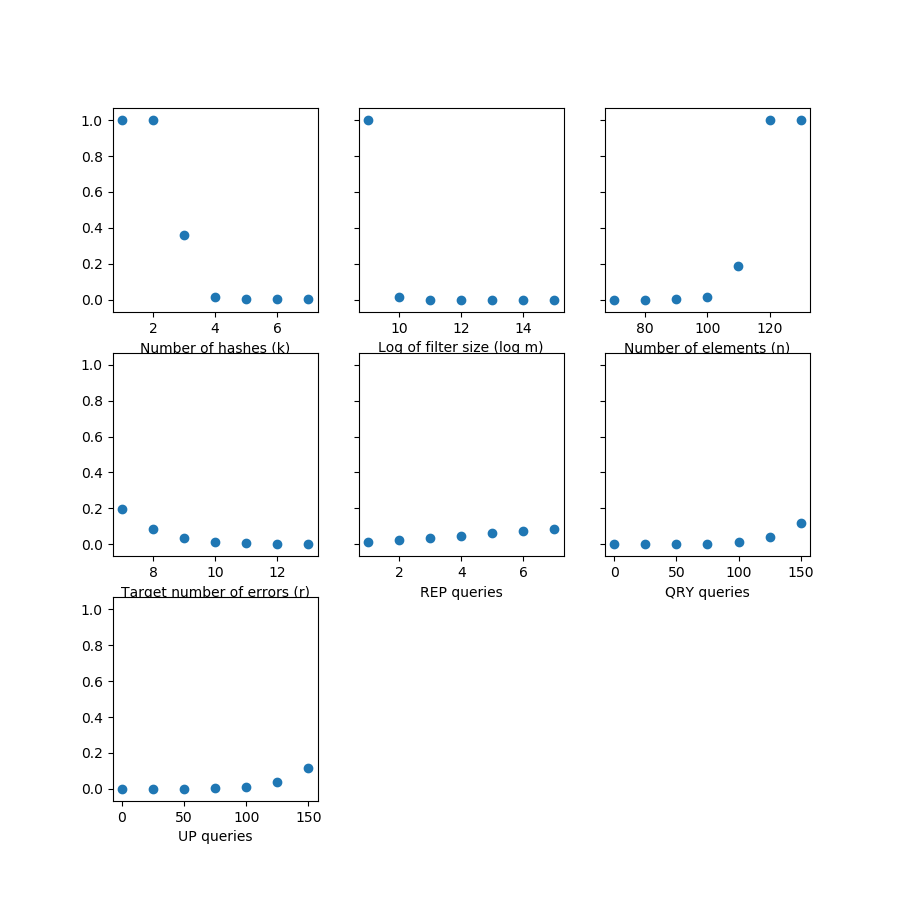
\includegraphics[scale=0.75]{BF_Fig}